\subsection{Constraints on \tesss Observing}
\label{sec:constraints_on_pointings}

When considering possible schedules for telescope pointings, the main
constraint is that the cameras must be directed approximately opposite
the Sun.  Specifically, the center of the combined fields-of-view is
ideally pointed within 15$^\circ$ in ecliptic longitude of the antisolar 
direction, and no more than 30$^\circ$ away.
%\todo[inline]{Roland: are these numbers still good? are they imposed by the sunshade? or solar panels? Some comment appreciated.} 
This enables the solar panels to collect
sufficient sunlight to power the spacecraft.
Fig.~\ref{fig:spacecraft_angles}) illustrates the geometry. The solar
panels are free to rotate about the $Y$-axis.

It is also important for the sunshade and 
spacecraft to block sunlight.
This constraint makes it difficult to remain pointed at a given field for more than two spacecraft orbits ($\approx$42 days). This is why \tess advances the fields of view by $\approx$$28^\circ$ east in ecliptic
longitude every lunar month, during the Primary Mission.  Another important consideration
is whether the Earth or Moon passes
through \tesss camera fields during a proposed pointing (see
Sec.~\ref{sec:earth_moon_crossings}), because these crossings are detrimental to high photometric precision.

In addition, the spacecraft has finite fuel reserves for necessary maneuvers.
These are expected to last at least 10 years [G. Ricker, priv.\ comm.].
Since the time horizon for this study is only 3 years, 
we do not consider the fuel reserves to be a constraint on the scenarios
we investigate.

\begin{figure}[!b]
	\centering
	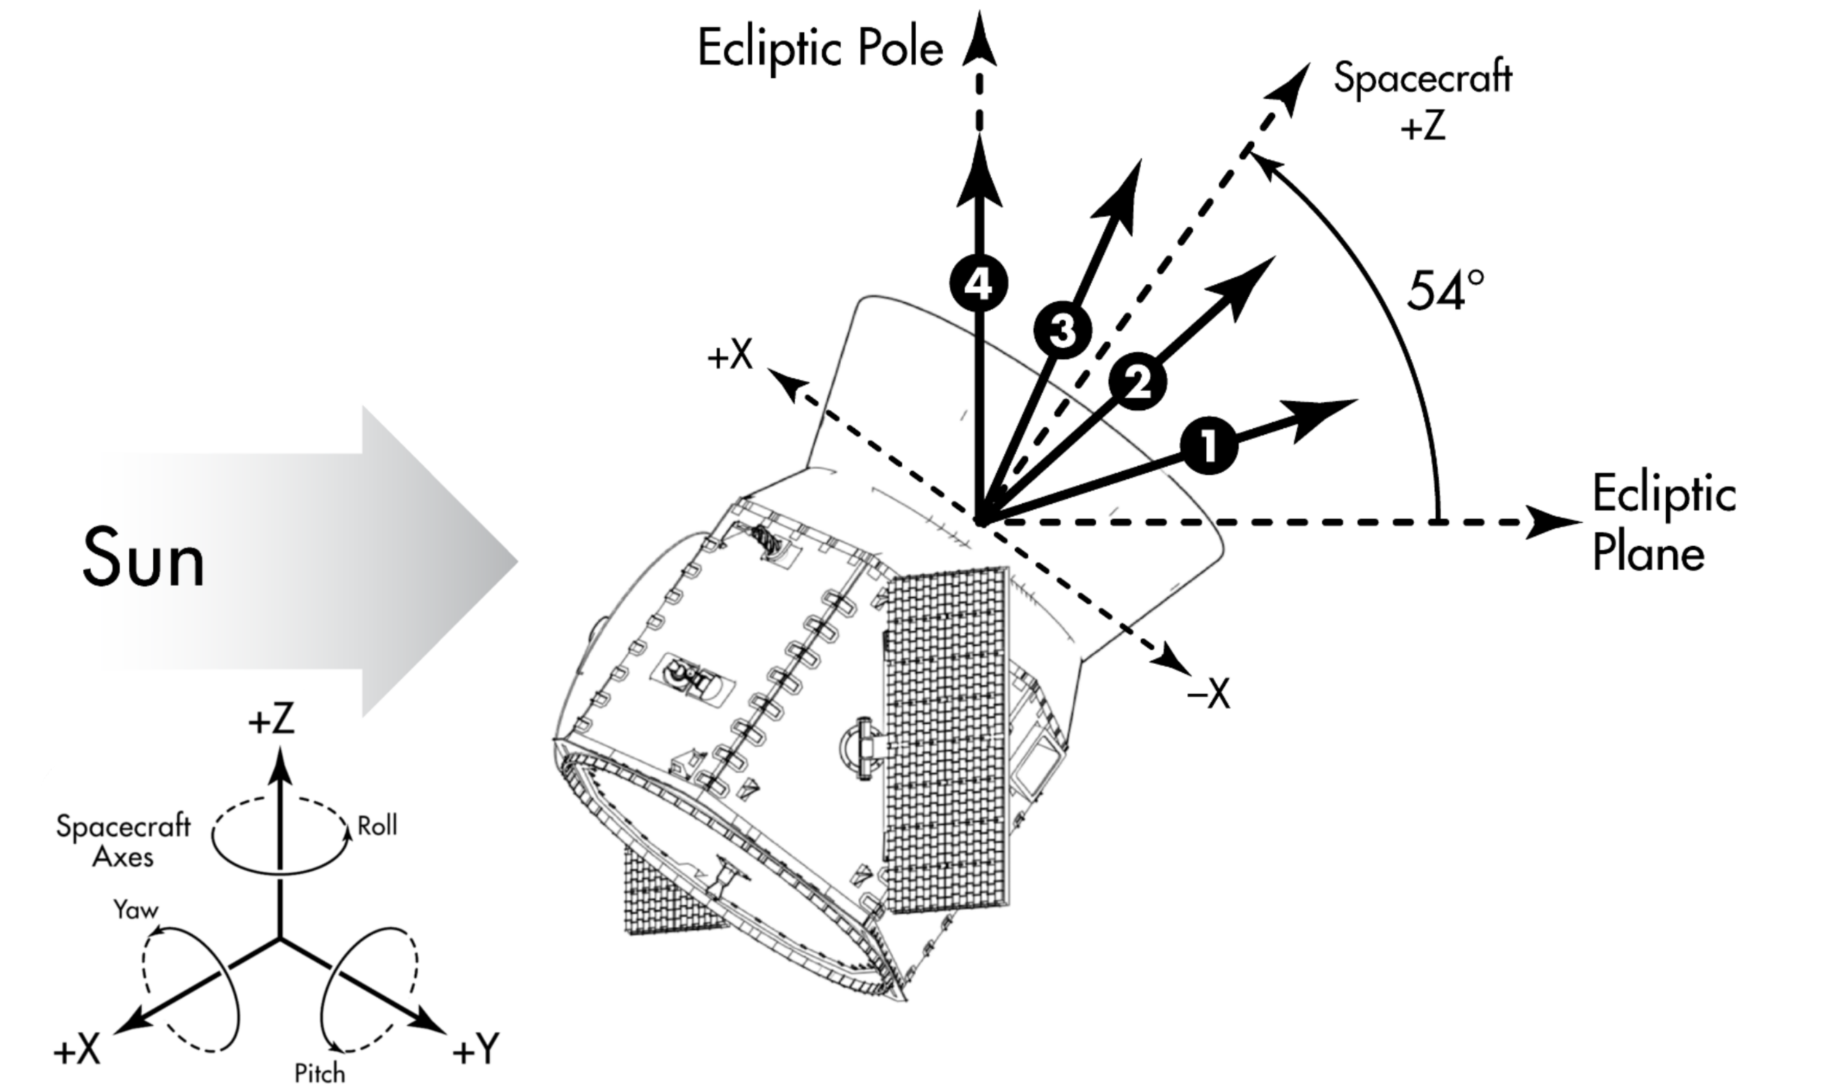
\includegraphics{figures/spacecraft_angles_corr.pdf}
	\caption{The spacecraft must point so that incident sunlight is collected 
		by the solar panels, and not the cameras. \tesss solar panels pitch 
		about the $+Y$ axis. (Adapted from Orbital ATK design document) }
	\label{fig:spacecraft_angles}
\end{figure}
